\documentclass[convert]{standalone}

\usepackage{tikz}
\pagestyle{empty}

% INT_AY22_L03_Fig06_Moving_ball_on_graph.png

\begin{document}
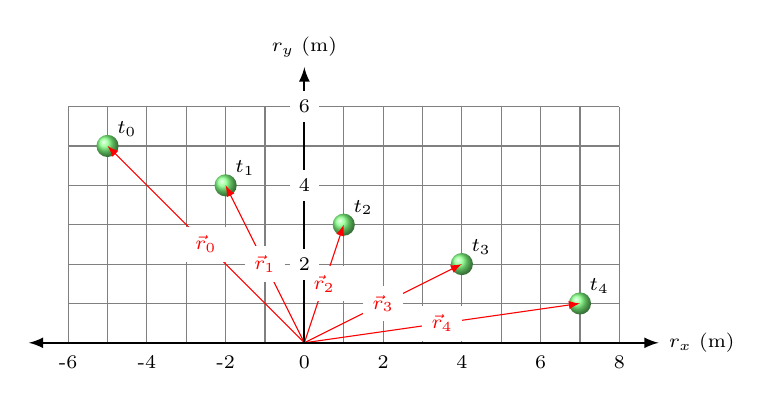
\begin{tikzpicture}[> = latex, font = \scriptsize]

	% Definitions
	
	\def\xi{-2.5}		% Initial x, y coordinates
	\def\yi{2.5}
	
	\def\vx{1.5}		% Velocity components
	\def\vy{-0.5}
	
	% Draw graph grid
	
	\draw [thin, gray, step = 0.5 cm] (-3, 0) grid (4, 3);
	
	% Draw ball
	
	\foreach \n in {0, 1, ..., 4}
	{
		\draw [ball color = green!50, draw = none] ({\xi + \n * \vx}, {\yi + \n * \vy}) circle (4 pt) node [above right] {$t_\n$};
		\draw [->, red] (0, 0) -- node [midway, fill = white] {${\vec r}_\n$} ({\xi + \n * \vx}, {\yi + \n * \vy});
	}
	
	% Draw axes + labels
	
	\draw [thick, <->] (-3.5, 0) -- (4.5, 0) node [right] {$r_x$ (m)};
	\draw [thick, ->] (0, 0) -- (0, 3.5) node [above] {$r_y$ (m)};
	
	\foreach \x in {-6, -4, ..., 8}
		\node at (0.5 * \x, -0.25) {\x};
		
	\foreach \y in {2, 4, 6}
		\node [fill = white] at (0, 0.5 * \y) {\y};
	
\end{tikzpicture}
\end{document}